\subsection{Inverted F-antenna}\label{sec:ifa_sim}

The inverted F-antenna (IFA) is modeled in Ansys HFSS as shown in \autoref{fig:ifa}. Its material is copper. It is positioned at the center of the TEM cell, mounted at the top surface. The excitation is a modal wave port. With a maximum dimension of 2.7\,mm, the antenna is electrically small for a frequency of up to 11.1\,GHz, at which it will be a tenth of the wavelength. In this simulation, the antenna is investigated for a frequency of 550\,MHz, therefore, its size is by far small enough.

\begin{figure}[h]
    \centering
    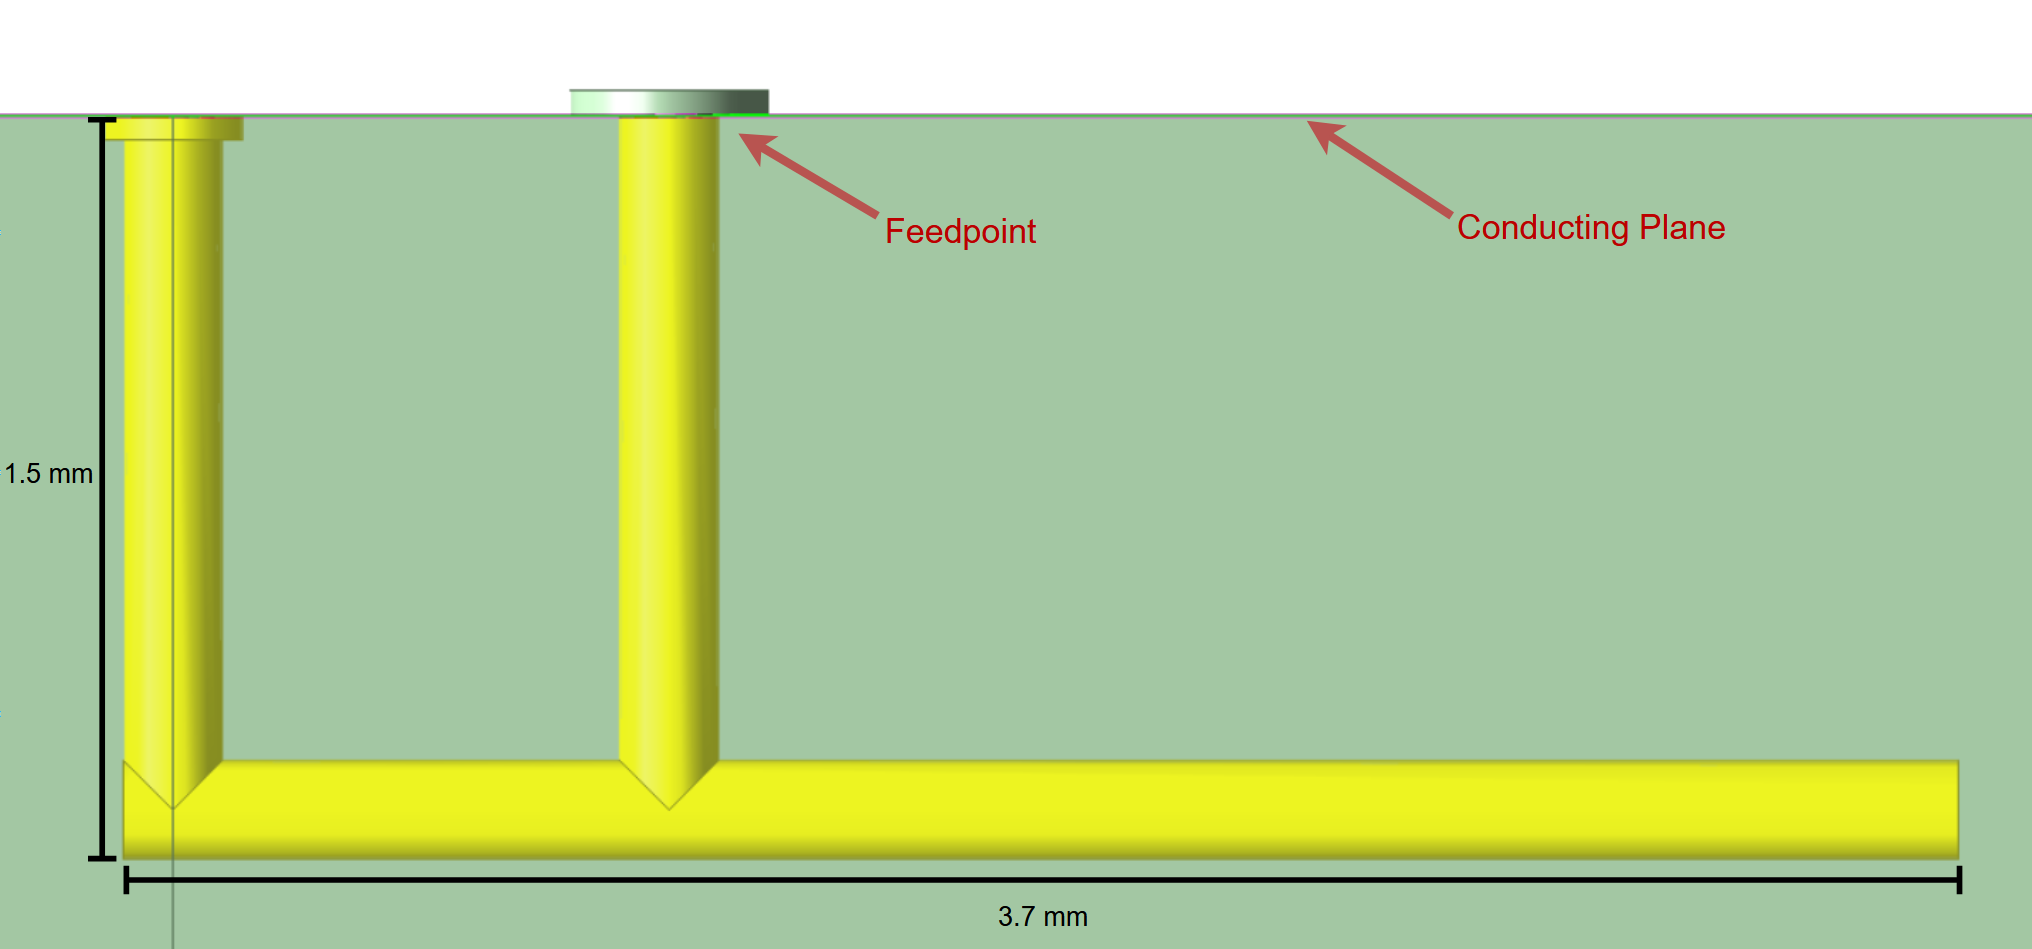
\includegraphics[width=0.7\linewidth]{Documentation//content//30_simulations//img/ifa.png}
    \caption{inverted F-antenna}
    \label{fig:ifa}
\end{figure}

The coupling between the antenna and the ports of the TEM cell are described by S-parameters. \autoref{fig:antenna_waveport1_sparams} and \autoref{fig:antenna_waveport1_sparams} show them for each ports, including the magnitude and phase. Specifically, the S-parameters at a frequency of 550\,MHz are marked, for which they are $S_{1\mathrm{A}}=3.337\cdot10^{-4}\cdot \mathrm{e}^{-\mathrm{i}\cdot151.85°}$ and $S_{2\mathrm{A}}=3.339\cdot10^{-4}\cdot \mathrm{e}^{\mathrm{i}\cdot40.76°}$. Note that the magnitude of the coupling is equal for each port, which is an inherent property of the electrically small antenna. Only the phase is different, which is due to the equivalent magnetic dipole.
 

\begin{figure}[h]
    \centering
    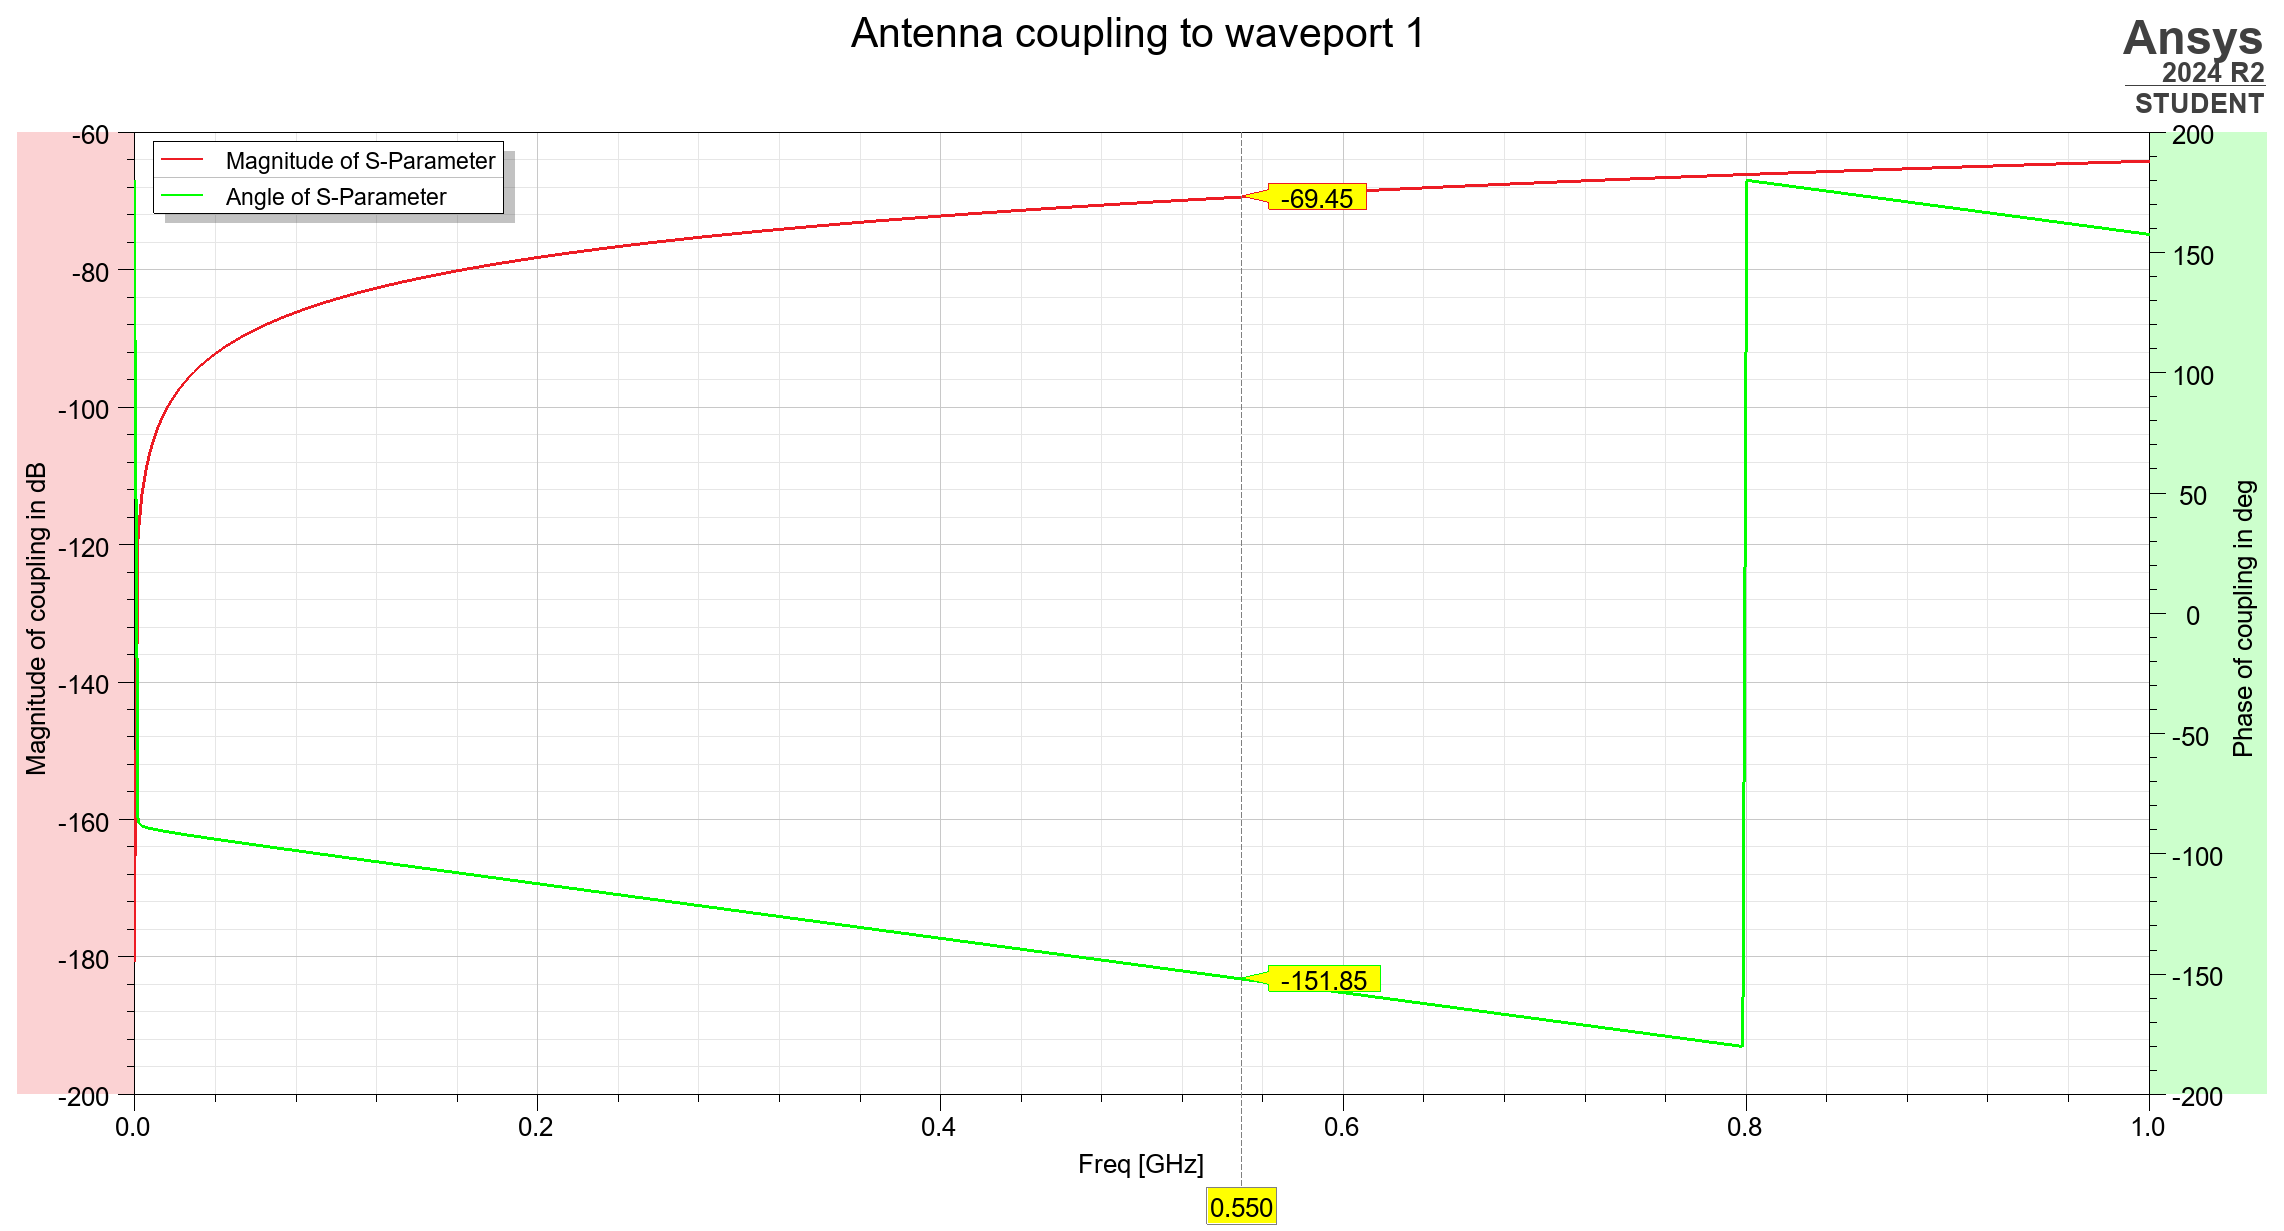
\includegraphics[width=1\linewidth]{Documentation//content//30_simulations//img/antenna_waveport1_sparams.png}
    \caption{S-Parameters describing coupling of antenna to waveport 1}
    \label{fig:antenna_waveport1_sparams}
\end{figure}

\begin{figure}[h]
    \centering
    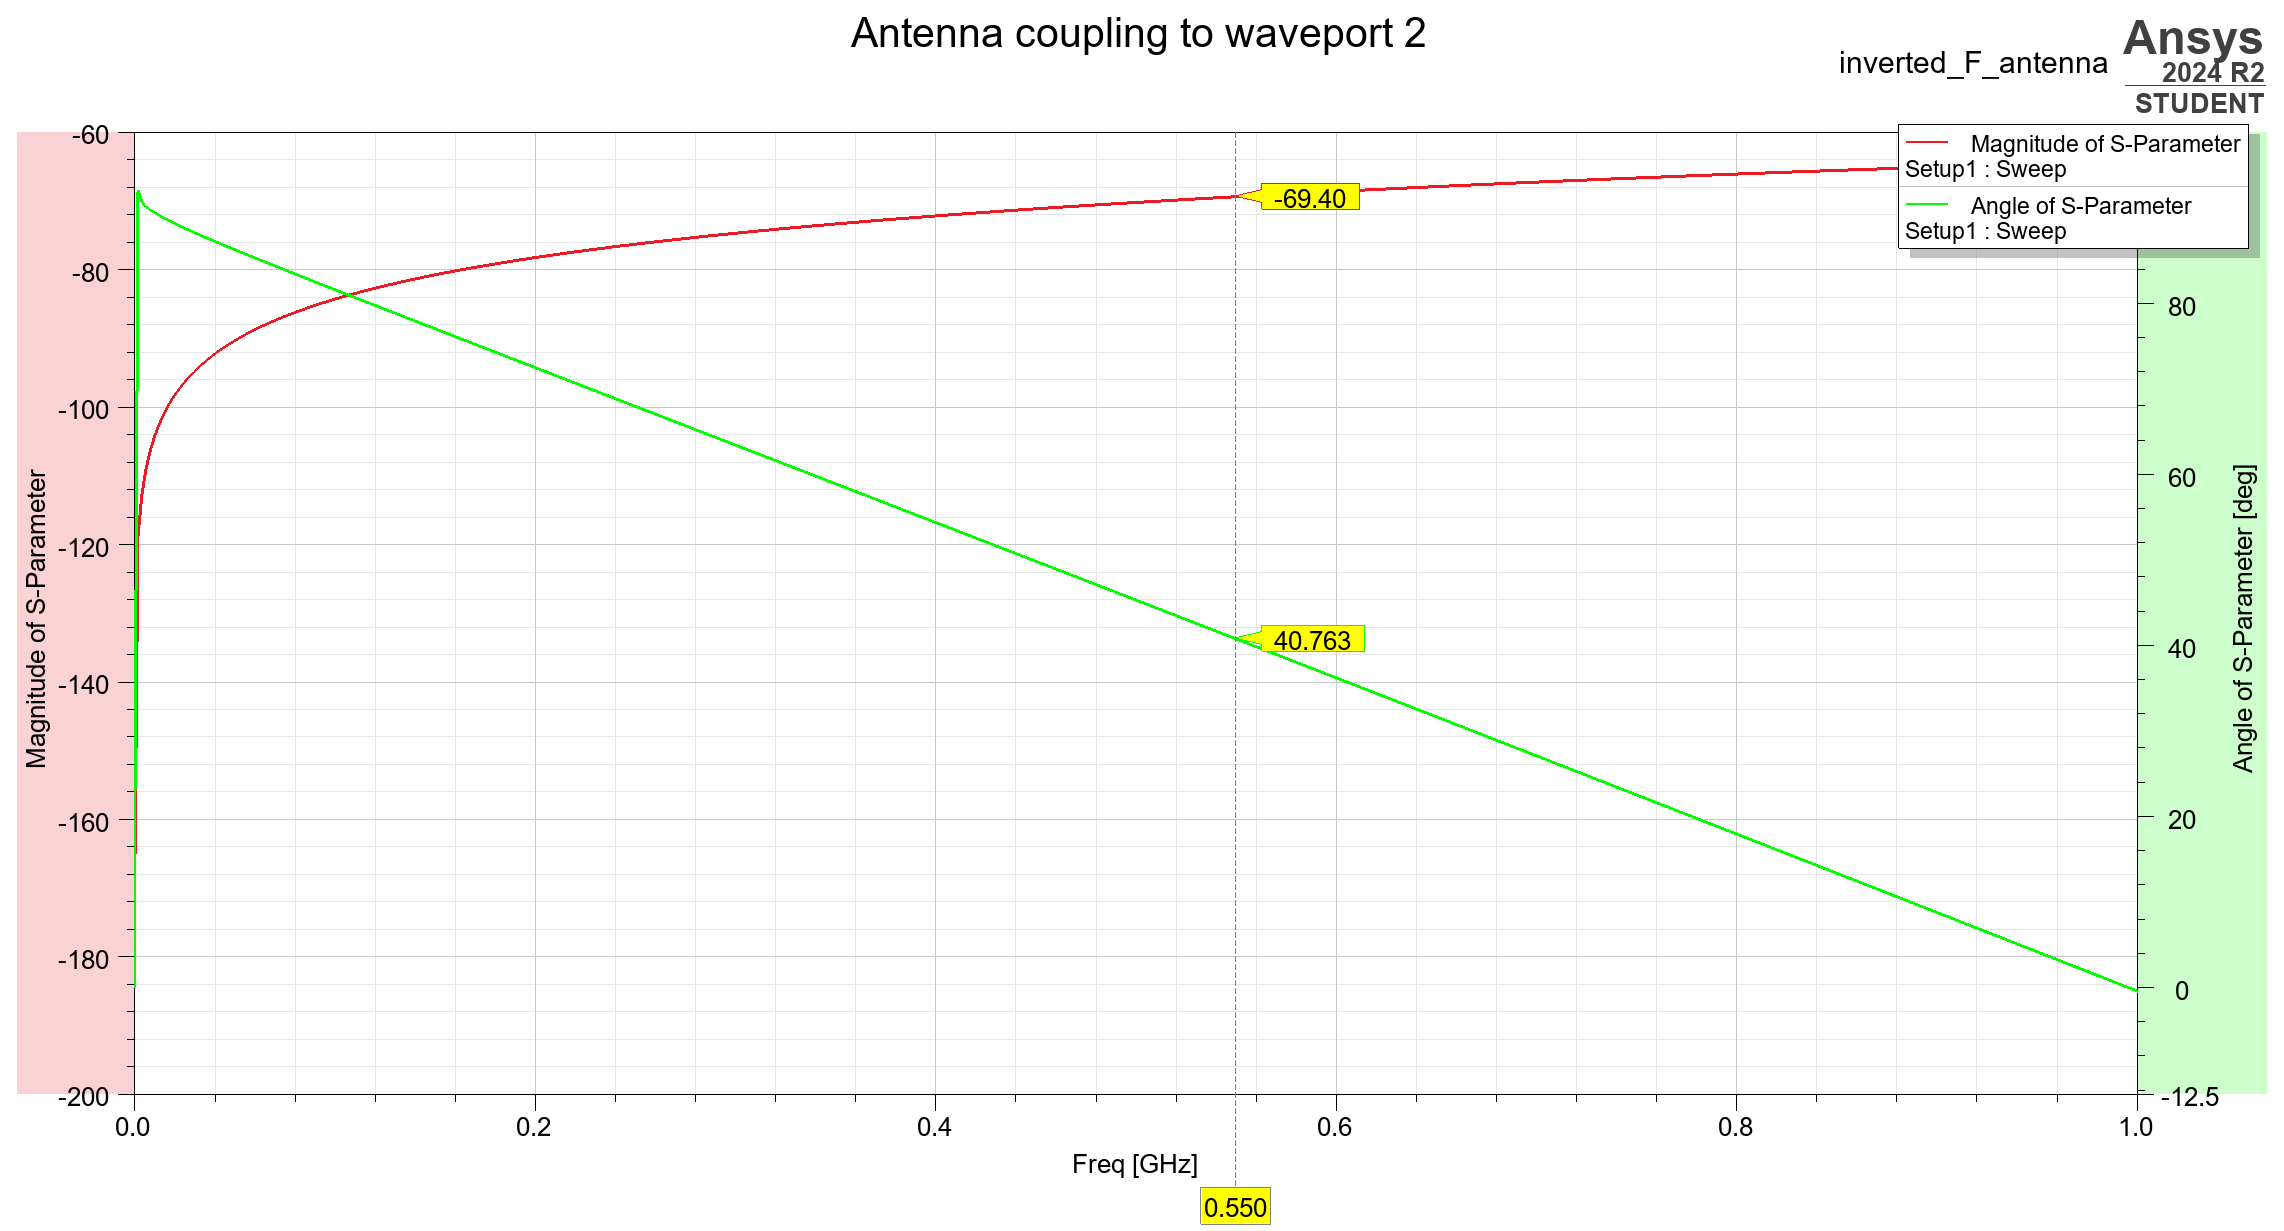
\includegraphics[width=1\linewidth]{Documentation//content//30_simulations//img/antenna_waveport2_sparams.png}
    \caption{S-Parameters describing coupling of antenna to waveport 2}
    \label{fig:antenna_waveport2_sparams}
\end{figure}

The measured electric field strength in z-direction at the center of the wave port is $E_{0,\mathrm{z}}=(-189.652 -\mathrm{i}\cdot66.529)\mathrm{\frac{V}{m}}$. It is much weaker in x- and y-direction, for which they will be ignored. The power at each output port is roughly 1\,W. Therefore, the amplitudes $|a|=|b|=\sqrt{P}=1\,\mathrm{\sqrt{W}}$ with a phase-shift of 167.39° between them, which will be needed to calculate the dipole moments according to \autoref{eqn:a_b_moments_simp}. The resulting dipole moments are displayed in \autoref{eqn:m_ez_ifa} and \autoref{eqn:m_my_ifa}.

\begin{align}
m_{\mathrm{ez}}&=1.099\cdot10^{-3}\cdot\mathrm{e}^{-\mathrm{i}\cdot124.99°}\mathrm{A\cdot m}\label{eqn:m_ez_ifa}\\
m_{\mathrm{my}}&=8.63\cdot10^{-4}\cdot\mathrm{e}^{-\mathrm{i}\cdot 124.99°}\mathrm{A\cdot m^2}\label{eqn:m_my_ifa}
\end{align}

Using \autoref{eqn:magn_current_curr_loop} the magnetic dipole moment can be expressed with a magnetic current. The resulting $m_{my,mag}$ is shown in \autoref{eqn:m_mymag_ifa}. Note that the phase shift between the magnetic and electric dipole moments $m_{\mathrm{ez}}$ and $m_{\mathrm{my,mag}}$ is exactly 90°, which creates a constructive interference pattern.

\begin{equation}
    m_{\mathrm{my,mag}}=\mathrm{i}m_{\mathrm{my}}\omega\mu_0=3.746\cdot\mathrm{e}^{-\mathrm{i}\cdot34.99°}\mathrm{V\cdot m}
    \label{eqn:m_mymag_ifa}
\end{equation}

Next, the antenna is replaced with those two dipole excitations in the center of the upper half of the TEM cell. The magnitude and phase of the fields is measured. The power going through each port is $\frac{1}{4}\,\mathrm{W}$. When doubling the excitations, the power reaches the desired $1\,\mathrm{W}$, but I could not find my error in my calculations yet. I suspect that somewhere there is a factor of two missing. The phase shift is determined by measuring the phase of the electric fields at the center of both output ports and comparing them. It is 165.32°, which is very close to the value with the real antenna.

\subsection{Center Fed Monopole Antenna}

The same simulation procedure is repeated with a center fed monopole antenna. The parameters are listed in \autoref{tab:center_fed_monopole_params} for the chosen frequency of 550\,MHz. Interestingly, the electric dipole moment increased proportionally to the antenna's height in z-direction compared to the IFA in \autoref{sec:ifa_sim}, while the magnetic dipole moment remained roughly equal due to the unchanged loop area.


\begin{table}[h]
    \centering
    \begin{tabular}{|c|c|}
        \hline
        Variable Name & Value\\\hline\hline
        $S_{1\mathrm{A}}$ & $3.51\cdot10^{-4}\cdot \mathrm{e}^{\mathrm{i}\cdot 48.86°}$\\\hline
         $S_{2\mathrm{A}}$&$3.49\cdot10^{-4}\cdot\mathrm{e}^{-\mathrm{i}\cdot 159.80°}$ \\\hline
         $E_{0,\mathrm{z}}$&$-189.652 -\mathrm{i}\cdot66.529\mathrm{\frac{V}{m}}$ \\\hline
         $m_{\mathrm{ez}}$&$2.463\cdot10^{-3}\cdot\mathrm{e}^{-\mathrm{i}\cdot74.8°}\cdot\mathrm{A\cdot m}$ \\\hline
         $m_{\mathrm{my}}$&$8.36\cdot10^{-4}\cdot\mathrm{e}^{-\mathrm{i}\cdot 74.8°}\cdot\mathrm{A\cdot m^2}$ \\\hline
         $m_{\mathrm{my,mag}}$&$3.6323\cdot\mathrm{e}^{\mathrm{i}\cdot15.1994}\cdot\mathrm{V\cdot m}$ \\\hline
    \end{tabular}
    \caption{Determined parameters of the center fed monopole antenna}
    \label{tab:center_fed_monopole_params}
\end{table}

